\section{Desarrollo}
	La actividad fue dividida en dos secciones, una encargada de realizar la simulación del juego de la vida y otra encargada de realizar la gráfica histórica de organismos vivos. Ambos programas fueron elaborados en Python 3.7, usando la librería tkinter y matlibplot respectivamente.
	\paragraph{Simulación del juego de la vida}
	El siguiente archivo ``gol.py'' muestra la implementación realizada del juego de la vida, los parámetros que recibe este programa es el tamaño del tablero y la probabilidad de organismos vivientes en el mismo. Ambos parámetros son enviados mediante la terminal como números enteros.

	Una vez ejecutado el programa, al usuario se le mostrá en pantalla el tablero con los organismos vivientes y las celdas vacías, así mismo se le permitirá configurar el color para los mismos. Además de tener la posibilidad de poder ingresar las reglas de supervivencia, muerte y nacimiento.

	\lstinputlisting[language=Python]{../gol.py}

	\paragraph{Gráfica de organismos vivos}
	Finalmente, se muestra el archivo ``graficar.py'' en el cual se realizó la implementación de la gráfica de organismos vivos que existen durante cada una de las generaciones de la simulación del juego de la vida. Los valores a graficar son la cantidad de organismos vivos y la generación a la que corresponden. Estos valores son leídos de un archivo .txt el cual contiene el histórico de organismos vivos, este archivo es actualizado cada que una generación transcurre en el juego de la vida. La gráfica se actualiza automaticamente cada segundo y fue elaborada usando matlibplot. 
	\lstinputlisting[language=Python]{../graficar.py}

	% \begin{figure}[H]
	% 	\begin{center}
	% 		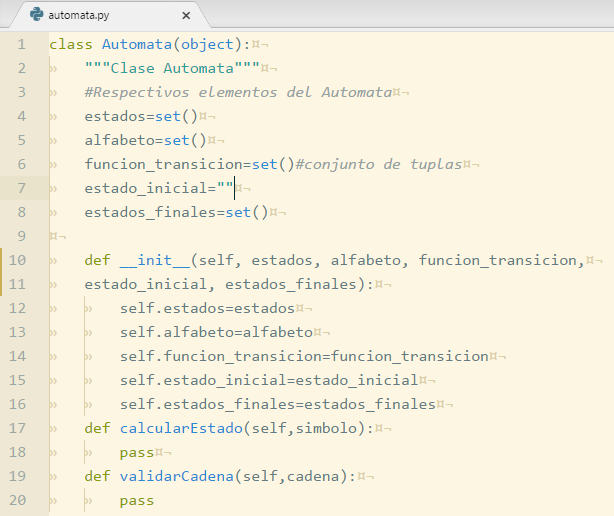
\includegraphics[width=15cm, height=12cm]{img/automata.png}
	% 		\caption{automata.py}
	% 		\label{fig:tablas}
	% 	\end{center}
	% \end{figure}